\documentclass[a4paper,11pt]{article}
\usepackage[utf8]{inputenc}
\usepackage[T1]{fontenc}
\usepackage{amsmath,amssymb}
\usepackage{graphicx}
\graphicspath{{figures/}}
\usepackage{booktabs}
\usepackage{array}
\usepackage[margin=1in]{geometry}
\usepackage[hidelinks]{hyperref}

% --- placeholder for figures whose image files are in the project zip ---
% Replace each \figph{...} with \includegraphics[width=...]{filename}
\newcommand{\figph}[1]{\begin{center}\fbox{\parbox[c][3.2cm][c]{0.86\textwidth}%
{\centering\itshape [figure placeholder]\\ #1}}\end{center}}

\title{Adapting the region-scale epidemic forest for city-level dengue
surveillance with quantified linkage uncertainty: a South Cotabato case study
with a preliminary cross-province transferability assessment in Region~12, Philippines}

\author{
Maria Yulita Trida Tahu$^{a}$, Nuning Nuraini$^{a}$, Kamal Sukandar$^{a,c}$,
Jayrold P. Arcede$^{b}$,\\ John Lemuel Dalisay$^{d}$, and Alah Baby C. Vingno$^{d}$
\\[6pt]
\small $^{a}$Department of Mathematics, Institut Teknologi Bandung, Indonesia \\
\small $^{b}$Department of Mathematics, Caraga State University, Butuan City, Philippines \\
\small $^{c}$Department of Mathematics and the Centre for the Mathematics of Precision Healthcare, \\
\small Imperial College London, London, UK \\
\small $^{d}$Integrated Provincial Health Office of South Cotabato (Department of Health partner), Philippines
}
\date{}

\begin{document}
\maketitle

\begin{abstract}
Dengue is endemic across the Philippines, yet outbreaks are strongly
heterogeneous in space and time: a few localities repeatedly ignite earlier and
carry higher burdens than their neighbours, and may seed transmission onward.
Reconstructing \emph{which} localities act as sources is central to resource
allocation, but epidemic-tree and epidemic-forest methods were formulated for
individual-level case data with precise residential coordinates, whereas
Philippine surveillance and response operate at the Local Government Unit (LGU)
scale mandated by Republic Act No.~11332. Building on the region-scale epidemic
forest of Nasution et al., which adapted the individual-level framework of Li et
al.\ to aggregated units and added case prevalence to spatial and temporal
proximity, we reconstruct dengue transmission at the LGU scale for the twelve LGUs
of South Cotabato and General Santos City over 2015--2020. Onset
dates are estimated per LGU from Richards-curve fits to smoothed cumulative
counts. In place of a fixed adjacency structure, admissible links are drawn from
a probabilistic distance-decay connectivity network, and the forest is
reconstructed as a Monte~Carlo ensemble over network realisations, summarised by
its modal structure with per-edge stability. Across three outbreak periods, the
ensemble does not support a single fixed transmission tree; what is stable is the
partition into sources and sinks. The provincial capital, Koronadal City, is the
dominant source in the first two periods and Banga in the third, while General
Santos City, the largest urban and coastal LGU, never seeds another locality in
any period. These source--sink findings are robust to the Strength-of-Linkage
weighting, to the decay rate and kernel form of the connectivity network, and to
replacing the probabilistic network with a deterministic adjacency; they also agree
with an independent spatio-temporal cluster analysis of the province. A preliminary application of the identical pipeline to three further
provinces of Region~12 recovers the same signature---an inland population or
administrative hub as the dominant source, with peripheral units terminal---in
each, indicating the pattern is a property of the method and settlement structure
rather than of one dataset. The results identify priority source LGUs for
intervention at the administrative scale at which response is deployed, while
making linkage uncertainty an explicit output.
\end{abstract}

\noindent\textbf{Keywords:} spatial--temporal transmission, dengue, region-scale
epidemic forest, connectivity network, ensemble uncertainty, Philippines

%======================================================================
\section{Introduction}
%======================================================================
Dengue fever remains a critical public health challenge in the Philippines, which
reported over 437{,}563 cases in 2019 alone, making it one of the highest-burden
countries in Southeast Asia \cite{Ong2022,Undurraga2017}. Region~12
(SOCCSKSARGEN) in Mindanao is particularly endemic for dengue \cite{Bravo2014},
with the disease exhibiting pronounced seasonal patterns and significant spatial
heterogeneity across municipalities and cities. Certain localities consistently
experience outbreaks earlier and with higher case loads than their neighbours
\cite{Edillo2015}, yet the spatial--temporal transmission pathways connecting
these areas remain poorly understood. Understanding which localities serve as
sources of transmission is essential for effective resource allocation and timely
intervention by regional health offices.

Traditional dengue surveillance and modelling approaches often focus on temporal
dynamics at aggregate scales, treating provinces or regions as homogeneous units
\cite{Morales2019,Polwiang2020}. Existing spatial approaches to dengue fall into
four families, none of which yields a directional, source-attributed hierarchy at
the administrative scale. Continuous-space mechanistic models based on
reaction--diffusion or cross-diffusion partial differential equations
\cite{Maidana2007,Maidana2008,Aguiar2022,Triska2022} describe travelling
wavefronts but not links between named units, and require mechanistic parameters
that routine surveillance rarely constrains. Movement- and network-based models
\cite{Lezama2018,Lourenco2013} represent \emph{potential} coupling between
patches but do not reconstruct realised transmission from case data.
Spatial-autocorrelation and clustering methods \cite{Nakhapakorn2006} detect
\emph{where} incidence concentrates but are non-directional, offering no
source-to-sink inference. Time-series and climate-correlational studies
\cite{Morales2019,Polwiang2020} characterise \emph{when} outbreaks occur and
their environmental drivers, but treat space only implicitly.

The epidemic-tree/forest lineage is the only family that recovers directional
parent--child structure. The concept of epidemic trees was introduced by Haydon
et al.\ \cite{Haydon2003} to analyse the 2001 UK foot-and-mouth outbreak, where
transmission linkages between farms---already spatial units rather than
individuals---were reconstructed from spatiotemporal proximity. Li et al.\
\cite{Li2019} formalised the epidemic forest as a framework for spatialising
epidemic modelling of communicable diseases; each tree represents a transmission
chain from a primary case, and the framework calculates the case reproduction
number ($R_t$) at global, tree-wise, and pixel-wise scales via kernel density
estimation. Li et al.\ applied it to individual-level dengue case data from
Guangzhou, China, where each node is a patient with a precise residential
location and onset time.

Regional surveillance in the Philippines, however, is organised differently. Under
Republic Act No.~11332 and its implementing rules \cite{RA11332,DOH2020IRR},
notifiable-disease reporting and the corresponding interventions are organised at
the LGU (city/municipality) level rather than at individual addresses, with the
Department of Health (DOH) and its local counterparts serving as the first line of
defence for epidemic detection and response. The LGU is therefore the unit of
\emph{action}, and a transmission hierarchy expressed in LGUs is directly
actionable in a way that an individual-level tree is not.

Most directly related to the present work is the region-scale epidemic forest of
Nasution et al.\ \cite{Nasution2024}, who adapted the individual-level framework
of Li et al.\ to aggregated administrative units, inferred onset with Richards
growth curves, and added case prevalence to the spatial and temporal terms of the
Strength-of-Linkage. Their construction restricts candidate parents to physically
adjacent regions through a fixed binary adjacency matrix and reports a single
deterministic forest (assessed across weighting combinations); consequently the
\emph{uncertainty} in each inferred link---which aggregation to administrative
units aggravates---is left unquantified, and their Discussion names the absence of
a richer inter-regional connectivity structure as a principal limitation.
Quantifying that linkage uncertainty, and supplying the missing connectivity
structure, is the central methodological aim of this paper.

We demonstrate the method on dengue transmission at the LGU scale across the twelve
LGUs of South Cotabato and General Santos City over 2015--2020---a window that
spans the region's 2016 epidemic and the 2019 national dengue epidemic
\cite{DOH2019epi}, during which SOCCSKSARGEN was among the hardest-hit regions---and
provide a preliminary generalisability check by applying the identical pipeline to
three further Region~12 provinces (Section~\ref{sec:crossprov}). Our contributions
are threefold.

\begin{enumerate}
    \item \textbf{A probabilistic connectivity layer and ensemble reconstruction
    for region-scale epidemic forests.} Where Nasution et al.\
    \cite{Nasution2024} restrict candidate parents to physically adjacent regions
    through a fixed binary adjacency matrix and report a single deterministic
    forest, we replace that fixed adjacency with a probabilistic distance-decay
    connectivity network (Eq.~\ref{eq:network}) and reconstruct the forest as a
    Monte~Carlo ensemble over network realisations, summarised by its modal
    structure with per-edge stability. This operationalises the inter-regional
    connectivity that Nasution et al.\ identified as missing, and makes linkage
    uncertainty---which aggregation aggravates---an explicit, quantified output.
    The distance-decay form is consistent with evidence that exponential kernels
    outperform Gaussian alternatives for short-range vector-borne transmission
    \cite{Ng2019,Routledge2021}.

    \item \textbf{The first reconstruction of a directional dengue transmission
    hierarchy among Philippine LGUs.} Across three outbreak periods we
    characterise which localities act as sources versus recipients and quantify
    each by an LGU reproduction number (Eq.~\ref{eq:rti}), recovering a stable
    inland-to-coastal source--sink tendency.

    \item \textbf{An assessment of translational utility at the response scale.}
    We show that ensemble city-scale forests identify stable early-onset,
    high-burden source LGUs---and, conversely, consistent terminal
    recipients---at the administrative scale to which RA~11332 assigns detection
    and response \cite{Nunes2014,Stoddard2013}.
\end{enumerate}

Table~\ref{tab:positioning} locates the present study among the four method
families and its epidemic-forest antecedents.

\begin{table}[htbp]
\centering
\caption{Positioning of the present study among spatial approaches to dengue.}
\label{tab:positioning}
\footnotesize
\setlength{\tabcolsep}{4pt}
\begin{tabular}{p{2.5cm}p{2.4cm}p{1.7cm}>{\centering\arraybackslash}p{1.8cm}>{\centering\arraybackslash}p{1.7cm}>{\centering\arraybackslash}p{2.0cm}}
\toprule
\textbf{Approach family} & \textbf{Representative works} & \textbf{Spatial unit} &
\textbf{Directional source?} & \textbf{Individual data?} &
\textbf{Uncertainty?} \\
\midrule
Continuous-space mechanistic (PDE) & \cite{Maidana2007,Aguiar2022,Triska2022} & continuous field & no & no & via parameters \\
Movement / network mechanistic & \cite{Lezama2018,Lourenco2013} & patches & prospective only & no & partial \\
Spatial autocorrelation / clustering & \cite{Nakhapakorn2006} & areal units & no & no & no \\
Time-series / climate & \cite{Morales2019,Polwiang2020} & aggregate region & no & no & partial \\
Epidemic trees / forest & \cite{Haydon2003} (farms); \cite{Li2019} (individuals); \cite{Nasution2024} (regions) & farms / persons / regions & yes & \cite{Li2019} yes & limited \\
\textbf{This study} & --- & \textbf{LGU} & \textbf{yes} & \textbf{no} & \textbf{yes (ensemble)} \\
\bottomrule
\end{tabular}
\end{table}

%======================================================================
\section{Materials and Methods}
%======================================================================
\subsection{Study area and data sources}
This study focuses on the province of South Cotabato and the adjacent independent
city of General Santos, in Region~12 (SOCCSKSARGEN), Mindanao, Philippines. The
study area comprises twelve LGUs: the eleven LGUs of South Cotabato---ten
municipalities and the component city of Koronadal (Banga, Koronadal City, Lake
Sebu, Norala, Polomolok, Santo Ni\~{n}o, Surallah, T'boli, Tampakan, Tantangan,
and Tupi)---together with General Santos City, the principal urban and coastal
centre and regional transportation hub. The
setting spans upland municipalities to the lowland urban centre, and is endemic
for dengue with seasonal outbreaks typically occurring during the rainy season.
Dengue surveillance follows the national reporting system, with data aggregated
at the LGU level before transmission to regional and national health offices. The
study window spans two of the region's most severe dengue seasons---the 2016
regional epidemic and the 2019 national epidemic, during which SOCCSKSARGEN dengue
cases rose by roughly $200\%$ and South Cotabato declared a state of calamity
\cite{DOH2019epi,DOH12_2019}.

Daily LGU-level dengue counts for 2015--2020 were drawn from the Department of
Health (DOH) Center for Health Development XII line-list for Region~12, a case
register recording each patient's municipality or city of residence and date of
onset; population figures are from the Philippine Statistics Authority (PSA), and
inter-LGU distances from municipal centroid coordinates. The reconstruction
pipeline below is \emph{agnostic to the particular province}: it takes a set of
LGUs with their counts, populations, and coordinates, so the same procedure applies
unchanged to any province. We therefore treat South Cotabato and General Santos
City as the primary study area---for which the full analysis is reported---and use
three further Region~12 provinces drawn from the same line-list (North Cotabato,
Sultan Kudarat, and Sarangani) as a preliminary cross-province transferability
assessment (Section~\ref{sec:crossprov}). Epidemic trajectories were smoothed and standardised
using the Richards growth curve \cite{Richards1959} applied to the DOH time series;
no individual-level simulation was performed. Table~\ref{tab:lgus} lists the twelve
primary-study LGUs with their populations.

\begin{table}[htbp]
\centering
\caption{The twelve LGUs of the study area, with 2015 populations and coordinates.}
\label{tab:lgus}
\small
\begin{tabular}{lrrrl}
\toprule
\textbf{LGU} & \textbf{Population} & \textbf{Latitude} & \textbf{Longitude} & \textbf{Type} \\
\midrule
Banga            & 89{,}164  & 6.4235 & 124.7734 & municipality \\
Koronadal City   & 195{,}398 & 6.5003 & 124.8435 & city (capital) \\
Lake Sebu        & 87{,}442  & 6.2248 & 124.7118 & municipality \\
Norala           & 44{,}642  & 6.5188 & 124.6567 & municipality \\
Polomolok        & 152{,}589 & 6.2142 & 125.0644 & municipality \\
Santo Ni\~{n}o   & 39{,}796  & 6.4380 & 124.6734 & municipality \\
Surallah         & 89{,}340  & 6.3756 & 124.7472 & municipality \\
T'boli           & 91{,}453  & 6.2136 & 124.8226 & municipality \\
Tampakan         & 41{,}018  & 6.4439 & 124.9272 & municipality \\
Tantangan        & 45{,}744  & 6.5632 & 124.7682 & municipality \\
Tupi             & 73{,}459  & 6.3310 & 124.9508 & municipality \\
General Santos City & 697{,}315 & 6.1200 & 125.1700 & city (urban centre) \\
\midrule
Total            & 1{,}647{,}360 & & & \\
\bottomrule
\end{tabular}

\smallskip
\noindent\small Population figures are from the 2015 Philippine Census
\cite{PSA2015}.
\end{table}

\subsection{Data preprocessing}
Daily time series for 2015--2020 were constructed for each LGU. Because the raw
daily counts are noisy, the merged daily series was smoothed with a
moving-average filter of span~60 days (which, following the standard convention,
operates with an effective odd span of 59 and a symmetric shrinking window at the
series edges). Agglomerative hierarchical clustering \cite{Johnson1967} was then
applied to reorder LGUs and reveal temporal coherence in a heatmap
(Fig.~\ref{fig:heatmap}): each LGU begins as its own cluster, and at each step the
two clusters minimising the squared distance between their mean case-series
(normalised by the sum of the two cluster means) are merged, until one cluster
remains; the resulting leaf order gives the row ordering. From the smoothed,
clustered series, three outbreak periods were retained (day indices $116$--$319$,
$510$--$800$, and $1550$--$1796$ relative to 1~January 2015). These windows were
identified by visual inspection of the smoothed regional case series and correspond
to the province's recognised epidemic years---the 2015, 2016--17, and 2019 outbreak
seasons, the last coinciding with the 2019 national dengue epidemic
\cite{DOH2019epi}; intervals without a sustained rise were excluded. We retain this
surveillance-anchored segmentation for interpretability and comparability with the
reporting periods used by the health office, and note that replacing it with an
algorithmic change-point procedure---for example, PELT or binary segmentation on the
smoothed incidence series---is a natural refinement for future work. Onset dates were
then estimated per LGU as described below.

\subsection{Mathematical methods}

\subsubsection{Onset date of outbreak}
An LGU is classified as infected once its cumulative case count exceeds a
population-dependent threshold. Following \cite{Nasution2024}, for LGU $i$ with
population $N_i$ the outbreak threshold is
\begin{equation}
\theta_i = 25 \cdot \frac{N_i}{100{,}000},
\label{eq:threshold}
\end{equation}
i.e.\ 25 cases per 100{,}000 population. The cumulative case series of each LGU is
fitted to the Richards (generalised-logistic) model \cite{Richards1959}
\begin{equation}
C(t) = K\left[1 + e^{-r\mu(t - \tau_i)}\right]^{-1/\mu},
\label{eq:richards}
\end{equation}
where $K$ is the final cumulative size, $r$ the per-capita growth rate, $\mu$ the
deviation exponent, and $\tau_i$ the inflection time. In implementation the
equivalent four-parameter form $C(t)=C_1\,[1+C_2\,e^{-C_3(t-C_4)}]^{-1/C_2}$ is
fitted, with $C_1=K$, $C_2=\mu$, $C_3=r\mu$; the coefficient $C_2$ only reparameterises
the inflection time, $\tau_i = C_4 + \ln(C_2)/C_3$. The onset day of LGU $i$ is
the first time at which the fitted curve reaches the threshold,
\begin{equation}
o_i = \min\{\, t : C(t) \ge \theta_i \,\},
\label{eq:onset}
\end{equation}
and onsets are normalised within each period by subtracting the earliest onset, so
that the earliest LGU has onset $0$. A smaller $o_i$ indicates an earlier
outbreak.

\subsubsection{Probabilistic connectivity network}
To represent admissible transmission links between LGUs, we place a probabilistic
edge between LGUs $i$ and $j$ with probability that decays with distance:
\begin{equation}
P_{ij} = e^{-\lambda\, d_{ij}},
\label{eq:network}
\end{equation}
where $d_{ij}$ is the (Euclidean, coordinate-based) distance between LGUs and
$\lambda>0$ controls the decay. A larger $\lambda$ yields a sparser, more
structured network. Unlike a fixed binary adjacency matrix \cite{Nasution2024},
Eq.~\ref{eq:network} defines a \emph{random} graph that is resampled to form an
ensemble (Sec.~\ref{sec:ensemble}). The exponential form is supported by evidence
that exponential kernels better represent short-range vector-borne dispersal than
Gaussian alternatives \cite{Ng2019,Routledge2021}.

The connectivity network has a single free parameter, the decay rate $\lambda$,
fixed at $\lambda=5$ throughout. Distances are measured in decimal degrees (one unit
$\approx 111$~km), so this value corresponds to an $e$-folding length of
$1/\lambda = 0.2^{\circ}\approx 22$~km and a half-probability distance of
$(\ln 2)/\lambda \approx 15$~km. That scale matches the short-range, locally
clustered dispersal characteristic of \emph{Aedes}-borne dengue, in which most
onward spread occurs between neighbouring communities and within daily-mobility
ranges rather than across an entire province \cite{Stoddard2009,Wesolowski2015}. At
this setting adjacent LGU centroids (typically $0.1$--$0.2^{\circ}$ apart) retain
edge probabilities of about $0.5$--$0.6$, whereas the most distant pairs
($\gtrsim 0.5^{\circ}$) fall below $0.1$, giving a sparse but connected
candidate-parent graph. Because $\lambda$ is not identifiable from aggregated
counts, we do not treat it as an estimated quantity; its influence---together with
the choice of an exponential rather than Gaussian kernel and a comparison against a
fixed binary adjacency matrix---is examined by the robustness analysis in
Section~\ref{sec:sens}.

\subsubsection{Strength of Linkage and parent assignment}
For a given child LGU $c$, the candidate parents are the LGUs connected to $c$ in
the current network realisation whose onset precedes $c$ by more than the
incubation period. Among candidates $j \in J_c$, the Strength of Linkage combines
three dimensionless criteria---spatial proximity, temporal proximity, and
prevalence---following Nasution et al.\ (\cite{Nasution2024}, their Eq.~5):
\begin{equation}
\mathrm{SoL}_{cj} =
\alpha\, \frac{1}{\tilde d_{cj}} +
\beta\, \frac{1}{\widetilde{\Delta o}_{cj}} +
(1-\alpha-\beta)\,\tilde p_{j} ,
\label{eq:sol}
\end{equation}
where $\tilde d_{cj} = d_{cj}/\min_{k\in J_c} d_{ck}$ and
$\widetilde{\Delta o}_{cj} = (o_c-o_j)/\min_{k\in J_c}(o_c-o_k)$ are the spatial
distance and temporal gap scaled by their candidate-set minima, and
$\tilde p_{j} = (p_j-p_c)/\max_{k\in J_c}\lvert p_k-p_c\rvert$ is the normalised
prevalence difference between candidate $j$ and the child at the child's onset
time. The parent of $c$ is the candidate maximising the Strength of Linkage,
\begin{equation}
\mathrm{parent}(c) = \arg\max_{j \in J_c} \mathrm{SoL}_{cj},
\label{eq:parent}
\end{equation}
so that spatially closer, temporally nearer, and higher-prevalence candidates are
preferred. Equation~\ref{eq:sol} is the maximised, inverse-distance Strength of
Linkage of Nasution et al.\ (\cite{Nasution2024}, their Eq.~5), adopted here so
that the region-scale (Jakarta) and city-scale (South Cotabato) studies share a
single linkage definition. The weights are set to the equal-weight baseline
$\alpha=\beta=\tfrac13$ (Nasution's combination~1); because they are not
identifiable from aggregated data, their influence on the reconstruction is
examined by sensitivity analysis in Section~\ref{sec:sens}.

\subsubsection{Ensemble reconstruction and edge stability}
\label{sec:ensemble}
Because aggregation removes individual resolution, a single reconstruction would
understate linkage uncertainty. We therefore resample the connectivity network
(Eq.~\ref{eq:network}) $M$ times; for each realisation the parent-assignment
procedure above produces one forest. For each child LGU we report the modal parent
across the $M$ realisations and its \emph{stability}---the fraction of
realisations in which that modal parent is selected---so that weakly determined
links are distinguished from robust ones.

The complete procedure is as follows. Given the per-LGU onsets $o_i$
(Eqs.~\ref{eq:threshold}--\ref{eq:onset}) and centroid coordinates:
\begin{enumerate}
\item \textbf{For each realisation} $m = 1,\dots,M$ (with a fixed random seed for
reproducibility):
  \begin{enumerate}
  \item draw a connectivity network by including each undirected edge $\{i,j\}$
  independently with probability $P_{ij}=e^{-\lambda d_{ij}}$ (Eq.~\ref{eq:network});
  \item visit the LGUs in random order; for each child $c$, form the candidate set
  $J_c$ of its network neighbours whose onset precedes $o_c$ by more than the
  incubation period;
  \item if $J_c\neq\varnothing$, set $\mathrm{parent}(c)=\arg\max_{j\in J_c}
  \mathrm{SoL}_{cj}$ (Eqs.~\ref{eq:sol}--\ref{eq:parent}); otherwise mark $c$ a
  primary case (no parent);
  \item record the resulting forest.
  \end{enumerate}
\item \textbf{Aggregate:} for each LGU take the modal parent across the $M$ forests
and its stability. On the modal forest, compute the LGU reproduction numbers
$R_{c,i}$ (Eq.~\ref{eq:rti}) and, per period, the global ratio $R_t$
(Eq.~\ref{eq:rt}).
\end{enumerate}
The full construction and normalisation of the Strength of Linkage
(Eq.~\ref{eq:sol}) is given in Appendix~\ref{app:sol}.

\subsubsection{Case reproduction ratio}
For a period $t$, the case reproduction ratio is
\begin{equation}
R_t = C_{pt}/P_t,
\label{eq:rt}
\end{equation}
where $P_t$ is the number of \emph{primary} (index) LGUs in period $t$---those with
no inferred parent---and $C_{pt}$ is the number of their descendants; because every
non-primary LGU has exactly one parent, $C_{pt}$ equals the number of non-primary
LGUs. Once the forest is reconstructed both counts are immediate, so $R_t$ follows
directly. The LGU reproduction number of LGU $i$, $R_{c,i}$, is its number of
\emph{direct} children (its out-degree) in the modal forest,
\begin{equation}
R_{c,i} = \big|\{\, c : \mathrm{parent}(c) = i \,\}\big|,
\label{eq:rti}
\end{equation}
measuring how many LGUs $i$ seeds; $R_t>1$ indicates growing spread and $R_t<1$
declining spread.

\subsubsection{Implementation, parameters, and reproducibility}
All parameters are collected in Table~\ref{tab:params}. Onsets are obtained by
fitting Eq.~\ref{eq:richards} to the cumulative series over each period, and the
merged daily series is smoothed with a span-60 (effective-59) moving average prior
to period selection. Distances $d_{ij}$ are Euclidean, computed between LGU
centroid coordinates. The ensemble uses a single fixed pseudo-random seed, so every
figure, table, and reported number is deterministically reproducible from the
inputs; the entire pipeline is provided as a documented notebook (see Code and data
availability).

\begin{table}[htbp]
\centering
\caption{Parameters and implementation settings used throughout.}
\label{tab:params}
\small
\begin{tabular}{p{6.2cm}p{2.0cm}p{5.2cm}}
\toprule
\textbf{Quantity} & \textbf{Symbol} & \textbf{Value / setting} \\
\midrule
Study window (daily) & --- & 1 Jan 2015 -- 31 Dec 2020 \\
Smoothing (moving average) & span & 60 (effective 59; symmetric shrinking window at edges) \\
Outbreak periods (day index from 2015-01-01) & --- & 116--319; 510--800; 1550--1796 \\
Outbreak threshold & $\theta_i$ & $25\cdot N_i/100{,}000$ (Eq.~\ref{eq:threshold}) \\
Onset model & --- & Richards curve (Eq.~\ref{eq:richards}) \\
Incubation period & --- & 5 days \\
Inter-LGU distance & $d_{ij}$ & Euclidean, centroid coordinates \\
Distance-decay rate & $\lambda$ & 5 (Eq.~\ref{eq:network}) \\
Strength-of-Linkage weights & $\alpha,\beta,1{-}\alpha{-}\beta$ & $\tfrac13,\tfrac13,\tfrac13$ (baseline; sensitivity in \S\ref{sec:sens}) \\
Ensemble size & $M$ & 5000 network realisations \\
Random seed & --- & fixed (0) \\
Software & --- & Python 3.10 (numpy, pandas, scipy, matplotlib) \\
\bottomrule
\end{tabular}
\end{table}

%======================================================================
\section{Results}
%======================================================================
\subsection{Empirical fitting of cumulative cases estimates the onset date}
The data comprise dengue cases from 1~January 2015 to 31~December 2020 for the
twelve LGUs of the study area. Time series are displayed as heatmaps in which the
horizontal axis is time (daily) and the vertical axis lists LGUs; brighter colours
indicate higher cumulative burden. When visual patterns do not reveal a clear
shift, hierarchical clustering reorders LGUs to highlight temporal coherence. We
fit the Richards curve to each LGU's cumulative series to obtain smooth
trajectories and estimate onset dates. Daily series display bell-shaped curves and
cumulative series display S-shaped curves. Three periods exhibiting clear shifts
in outbreak intensity were retained for onset and propagation analysis.

\begin{figure}[htbp]
\centering
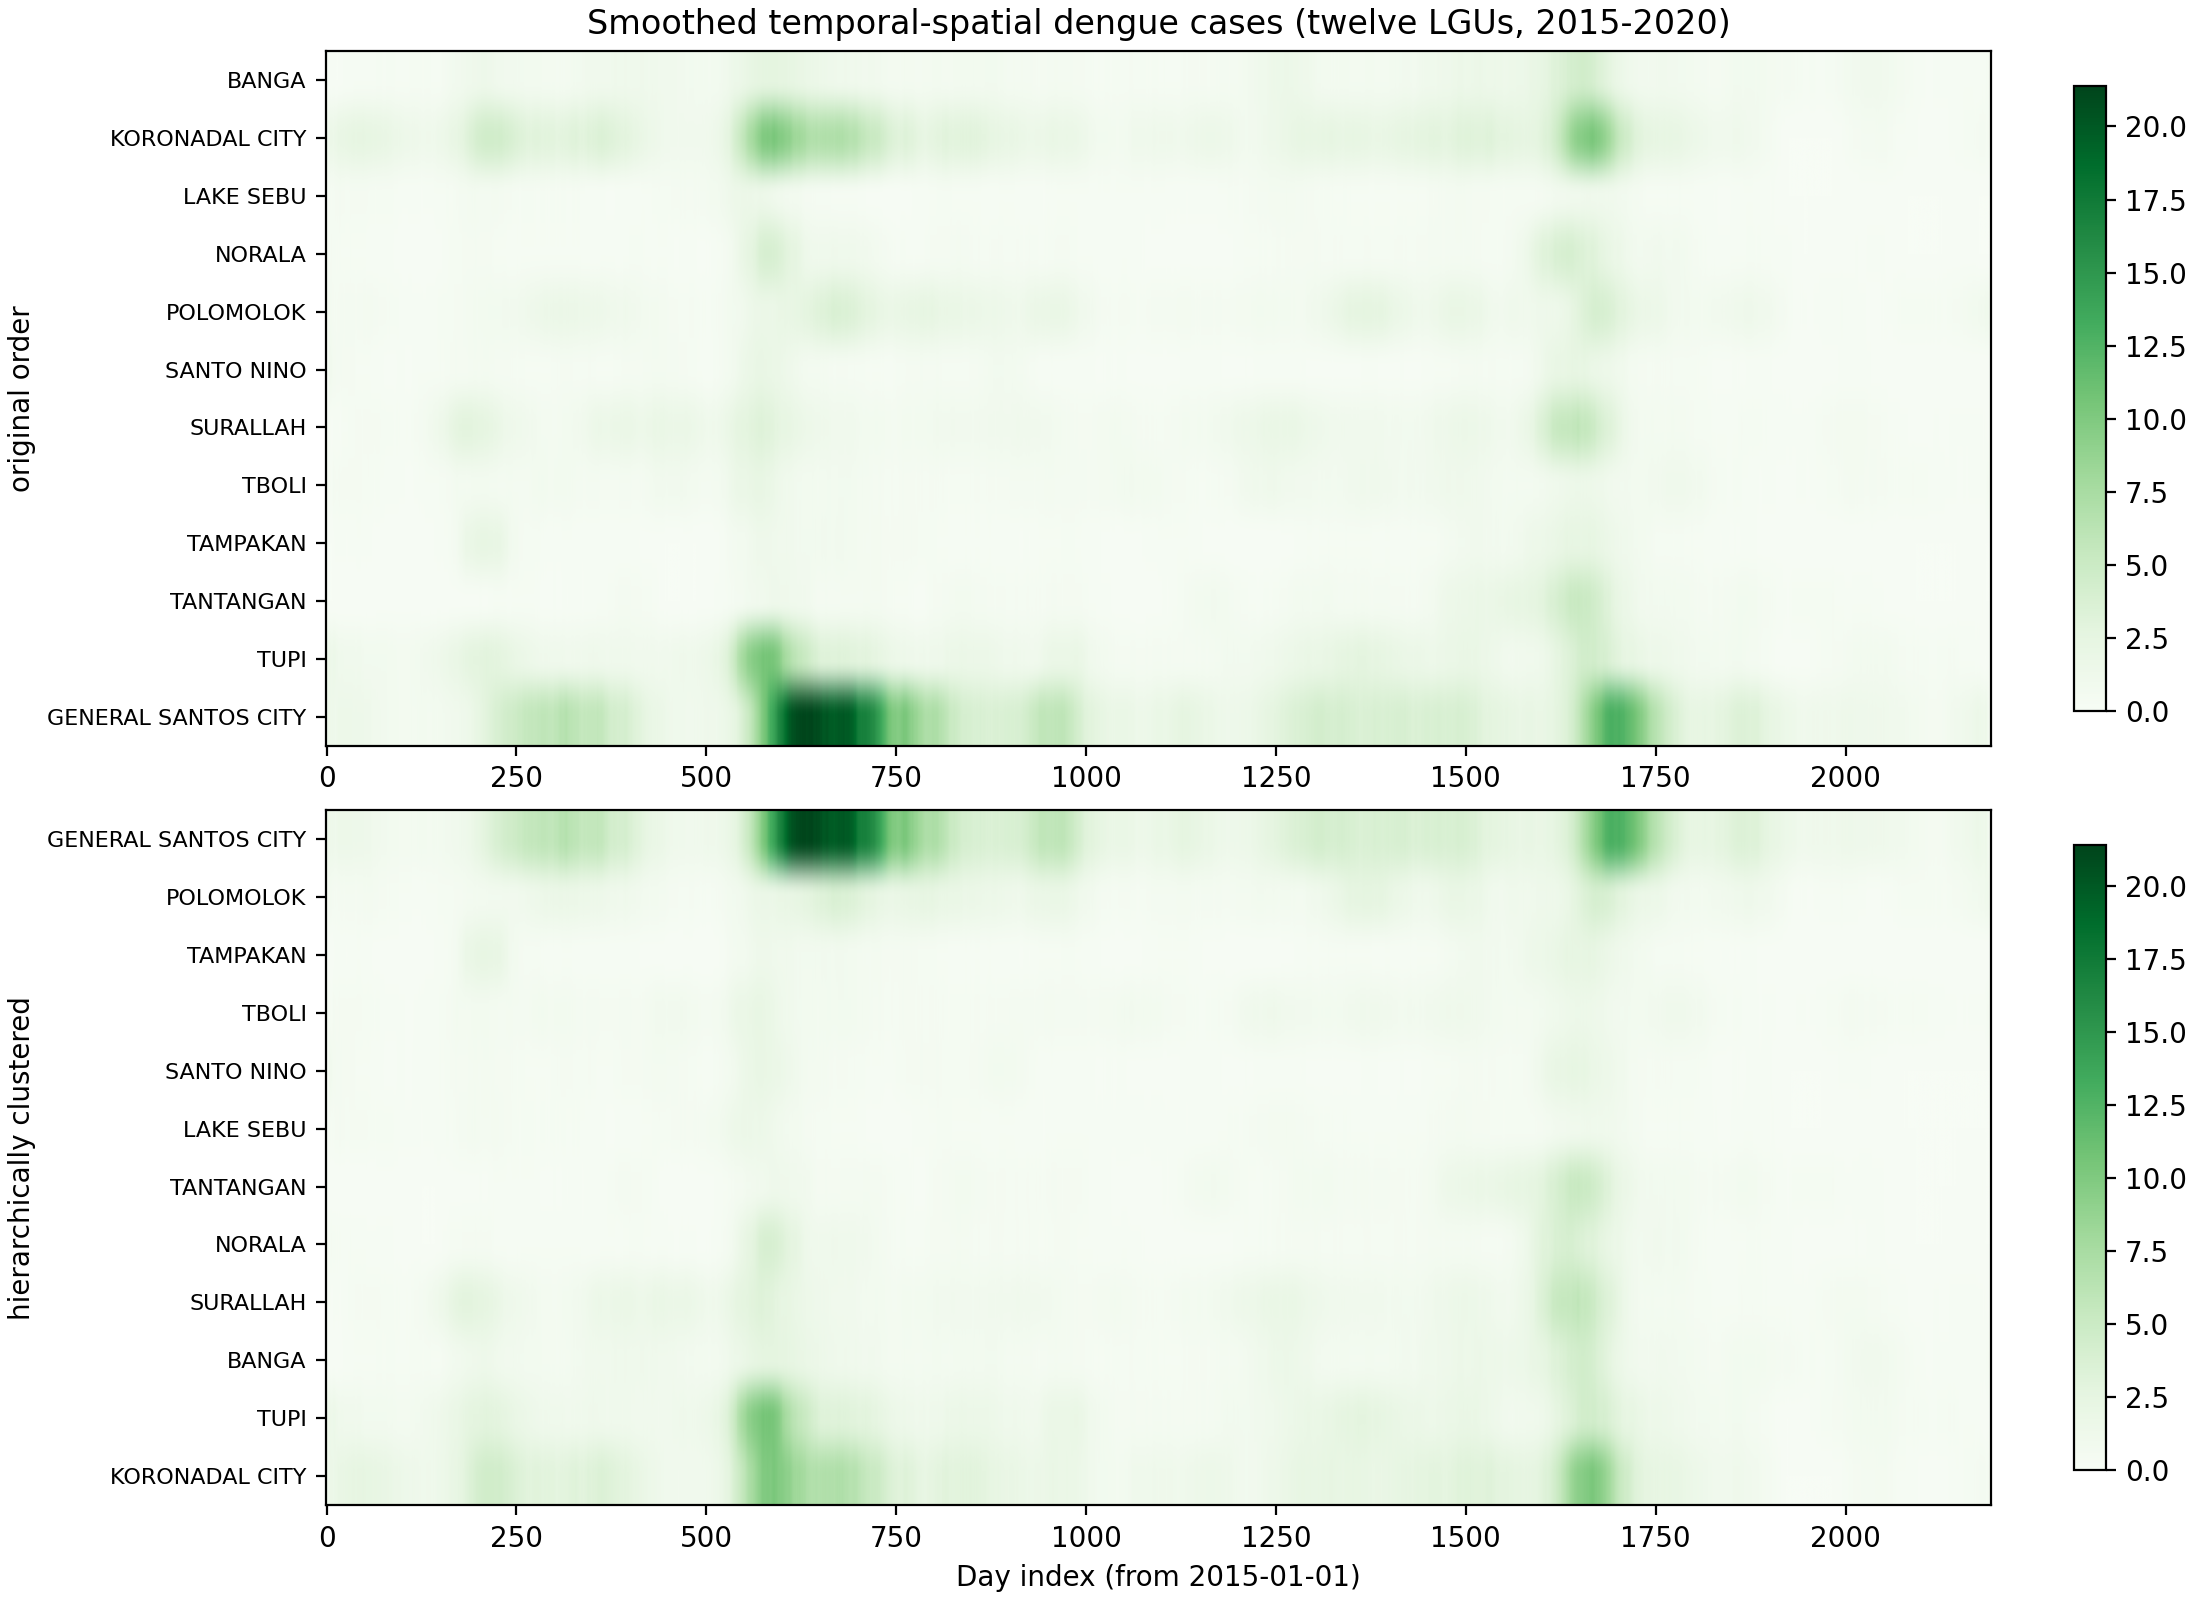
\includegraphics[width=0.9\textwidth]{heatmap_two_panel.png}
\caption{Heatmap and smoothed temporal--spatial series of dengue cases for the
twelve LGUs, 2015--2020. Top: LGUs in their original order; bottom: LGUs reordered
by hierarchical clustering to highlight temporal coherence. Brighter colours
indicate higher cumulative burden.}
\label{fig:heatmap}
\end{figure}

\subsection{Burden LGUs tend to have earlier onset}
Per-capita dengue incidence (cases per 100{,}000 population) decreases
consistently as onset time increases across the outbreak periods (pooled
standardised Pearson $r=-0.67$; see Fig.~\ref{fig:onset}); the association is
weaker and dominated by population size when raw case counts are used instead.
Taken together, the evidence suggests that LGUs with the earliest onsets
tend to accumulate higher burdens and may seed infections to other areas via human
mobility \cite{Stoddard2009,Wesolowski2015}. Under this interpretation,
early-onset, high-burden LGUs are plausible priority targets for intervention.
While the analysis does not identify exact transmission routes, it supports
focusing control on early-onset hubs.

\begin{figure}[htbp]
\centering

\includegraphics[width=0.72\textwidth]{onset_vs_cases.png}
\caption{Standardised association between onset time and per-capita dengue
incidence (cases per 100{,}000 population) across the three outbreak periods. Each
point is an LGU within a period; both axes are standardised within period. The
negative slope (pooled Pearson $r=-0.67$) indicates that earlier-onset LGUs tend
to accumulate higher incidence.}
\label{fig:onset}
\end{figure}

\subsection{Ensemble forests identify stable inland sources and a consistently
terminal coastal centre}
For each outbreak period we reconstruct the epidemic forest as an ensemble over
$M=5000$ network realisations and report, for every LGU, the modal parent together
with its stability and the resulting LGU reproduction number $R_{c,i}$
(Eq.~\ref{eq:rti}). Table~\ref{tab:stability} gives the modal parent and stability
by period; Table~\ref{tab:rc} gives $R_{c,i}$.

\begin{table}[htbp]
\centering
\caption{Modal parent and its stability (fraction of $5000$ realisations selecting
it) by period. ``primary'' denotes an inferred primary case (no parent).}
\label{tab:stability}
\small
\begin{tabular}{lccc}
\toprule
\textbf{Child LGU} & \textbf{Period 1} & \textbf{Period 2} & \textbf{Period 3} \\
\midrule
Banga            & Koronadal (60\%)  & Koronadal (60\%)  & Tantangan (48\%) \\
Koronadal City   & Surallah (45\%)   & primary (63\%)    & Banga (46\%) \\
Lake Sebu        & T'boli (58\%)     & T'boli (32\%)     & T'boli (38\%) \\
Norala           & Koronadal (40\%)  & Koronadal (40\%)  & Banga (47\%) \\
Polomolok        & Tupi (44\%)       & Tupi (45\%)       & Tupi (28\%) \\
Santo Ni\~{n}o   & Surallah (62\%)   & Surallah (62\%)   & Koronadal (41\%) \\
Surallah         & primary (65\%)    & primary (65\%)    & Banga (77\%) \\
T'boli           & Tupi (28\%)       & Tupi (41\%)       & Surallah (30\%) \\
Tampakan         & Koronadal (61\%)  & Koronadal (61\%)  & primary (63\%) \\
Tantangan        & Koronadal (61\%)  & Koronadal (61\%)  & primary (100\%) \\
Tupi             & primary (100\%)   & primary (100\%)   & Banga (37\%) \\
General Santos City & Polomolok (33\%) & primary (34\%)  & Polomolok (40\%) \\
\bottomrule
\end{tabular}
\end{table}

\begin{table}[htbp]
\centering
\caption{LGU reproduction number $R_{c,i}$ (number of LGUs seeded in the modal
forest) by period.}
\label{tab:rc}
\small
\begin{tabular}{lcccl}
\toprule
\textbf{LGU} & \textbf{P1} & \textbf{P2} & \textbf{P3} & \textbf{Role} \\
\midrule
Koronadal City   & 4 & 4 & 1 & dominant hub, P1--P2 (capital) \\
Tupi             & 2 & 2 & 1 & consistent source; primary P1--P2 \\
Banga            & 0 & 0 & 4 & dominant hub, P3 \\
Surallah         & 2 & 1 & 1 & primary, P1--P2 \\
T'boli           & 1 & 1 & 1 & \\
Polomolok        & 1 & 0 & 1 & \\
Tantangan        & 0 & 0 & 1 & primary, P3 \\
Lake Sebu        & 0 & 0 & 0 & never a source \\
Norala           & 0 & 0 & 0 & never a source \\
Santo Ni\~{n}o   & 0 & 0 & 0 & never a source \\
Tampakan         & 0 & 0 & 0 & never a source; primary, P3 \\
General Santos City & 0 & 0 & 0 & never a source (always terminal) \\
\bottomrule
\end{tabular}
\end{table}

The ensemble does not support a single fixed hierarchy across periods: only two
links---Lake~Sebu $\leftarrow$ T'boli and Polomolok $\leftarrow$ Tupi---are the
modal parent in all three periods. What is stable is the identity of sources and
sinks. Koronadal~City, the provincial capital, is the dominant source in
Periods~1 and 2, seeding four LGUs in each ($R_{c}=4$); in Period~3 the dominant
hub shifts to Banga ($R_{c}=4$). Tupi is a consistent secondary source
($R_{c}=2,2,1$) and an isolated primary in Periods~1 and 2 (stability $100\%$),
while Surallah is a primary in Periods~1 and 2 (stability $65\%$). Conversely,
General Santos City---the principal urban and coastal LGU---never seeds another
locality in any period ($R_{c}=0$ throughout), together with Lake~Sebu, Norala,
Santo~Ni\~{n}o and Tampakan. Several individual links are weakly determined (modal
stability below $40\%$, e.g.\ the parent of T'boli in Period~1), and we therefore
base interpretation on the high-stability sources and sinks rather than on any
single reconstructed tree. At the period level, the number of inferred primaries
and children gives global reproduction ratios (Eq.~\ref{eq:rt}) of $5.0$, $2.0$,
and $5.0$ for Periods 1--3, respectively. Taken together, the ensemble indicates a
directional tendency from inland population and administrative hubs toward the
coastal urban centre.

\begin{figure}[htbp]
\centering

\includegraphics[width=0.62\textwidth]{forest_period1.png}\\[3pt]

\includegraphics[width=0.62\textwidth]{forest_period2.png}\\[3pt]

\includegraphics[width=0.62\textwidth]{forest_period3.png}
\caption{Modal epidemic forests for Periods 1--3 (top to bottom) over the study
area, from the Monte-Carlo ensemble (consistent with Tables~\ref{tab:stability}
and~\ref{tab:rc}). Node size and colour scale with cumulative burden; arrows show
the modal parent-to-child direction of transmission, with arrow width proportional
to edge stability.}
\label{fig:forest}
\end{figure}

\subsection{Robustness analyses}
\label{sec:sens}
\subsubsection*{Strength-of-Linkage weights}
The weights $\alpha$ (spatial), $\beta$ (temporal), and $1-\alpha-\beta$
(prevalence) in Eq.~\ref{eq:sol} are not identifiable from the aggregated data,
because no ground-truth transmission network is observed against which to fit them.
Rather than tuning them, we assess how far the reconstruction depends on them by
recomputing the ensemble for the eight weight combinations of Nasution et al.\
(\cite{Nasution2024}, their Table~1), which span equal weighting to prevalence- and
temporal-dominant regimes (Table~\ref{tab:sens}). The main findings are stable
across this range: the global reproduction ratios remain $5.0/2.0/5.0$ in seven of
the eight combinations (and $5.0/2.0/3.0$ in the most prevalence-dominant one);
General~Santos~City never seeds another locality ($R_{c}=0$) in \emph{every}
combination and period; Koronadal~City is the dominant source in Periods~1 and~2 in
seven of eight combinations; and Banga is the Period-3 hub in five of eight
(Tantangan otherwise). Mean modal stability varies only within $0.48$--$0.56$. We
therefore report the equal-weight baseline $\alpha=\beta=\tfrac13$ in the main
analysis, noting that the source--sink partition and the reproduction ratios are
not an artefact of the weight choice.

\begin{table}[htbp]
\centering
\caption{Sensitivity of the reconstruction to the Strength-of-Linkage weights
$(\alpha,\beta,1{-}\alpha{-}\beta)$, across the eight combinations of Nasution
et al.\ (their Table~1; combination~1 is the equal-weight baseline used in the main
analysis). ``Dominant source'' is the LGU with the largest $R_{c}$ in each period
(value in parentheses).}
\label{tab:sens}
\footnotesize
\setlength{\tabcolsep}{4pt}
\begin{tabular}{lc>{\raggedright\arraybackslash}p{5.6cm}cc}
\toprule
\textbf{$(\alpha,\beta,1{-}\alpha{-}\beta)$} & \textbf{Mean stab.} &
\textbf{Dominant source P1 / P2 / P3} & \textbf{GenSan $R_c$} & \textbf{$R_t$} \\
\midrule
$(\tfrac13,\tfrac13,\tfrac13)$ & 0.53 & Koronadal (4) / Koronadal (4) / Banga (4) & 0/0/0 & 5/2/5 \\
$(0.10,0.45,0.45)$ & 0.52 & Koronadal (4) / Koronadal (4) / Banga (4) & 0/0/0 & 5/2/5 \\
$(0.45,0.10,0.45)$ & 0.53 & Koronadal (4) / Surallah (3) / Tantangan (3) & 0/0/0 & 5/2/5 \\
$(0.25,0.50,0.25)$ & 0.55 & Koronadal (3) / Koronadal (4) / Banga (4) & 0/0/0 & 5/2/5 \\
$(0.15,0.70,0.15)$ & 0.53 & Banga (2) / Koronadal (3) / Banga (4) & 0/0/0 & 5/2/5 \\
$(0.45,0.45,0.10)$ & 0.56 & Koronadal (3) / Koronadal (3) / Banga (4) & 0/0/0 & 5/2/5 \\
$(0.25,0.25,0.50)$ & 0.52 & Koronadal (4) / Koronadal (4) / Tantangan (3) & 0/0/0 & 5/2/5 \\
$(0.15,0.15,0.70)$ & 0.48 & Koronadal (4) / Koronadal (3) / Tantangan (3) & 0/0/0 & 5/2/3 \\
\bottomrule
\end{tabular}
\end{table}

\subsubsection*{Decay rate, kernel form, and network type}
The connectivity model introduces one free parameter, the decay rate $\lambda$
(Eq.~\ref{eq:network}), together with a choice of kernel. We therefore repeated the
full ensemble reconstruction while (i) varying $\lambda$ over an order of magnitude,
(ii) replacing the exponential kernel with a Gaussian one matched at its
half-probability distance, and (iii) replacing the probabilistic network with a fixed
binary adjacency matrix---LGUs joined when their centroids lie within a distance
chosen to match the mean degree of the $\lambda=5$ network---which reproduces the
deterministic set-up of Nasution et al.\ \cite{Nasution2024}. Table~\ref{tab:kernrob}
summarises the outcome and Fig.~\ref{fig:kernrob} plots the leading reproduction
numbers against $\lambda$.

The qualitative structure is remarkably stable. General~Santos~City has $R_{c}=0$ in
\emph{every} setting and period, and Koronadal~City (Periods~1--2) and Banga
(Period~3) remain the dominant sources throughout---under all six decay rates, under
the Gaussian kernel, and under the deterministic adjacency. What $\lambda$ controls is
the \emph{density} of the candidate network, and hence the magnitude of the global
reproduction ratios: a small $\lambda$ yields a dense graph in which almost every LGU
is seeded ($R_t\approx 11$), whereas a large $\lambda$ starves the graph of admissible
links ($R_t\to 0$); the baseline $\lambda=5$ occupies an intermediate regime with
$R_t = 5/2/5$. Notably, the deterministic adjacency recovers the same dominant sources
and the same $R_t = 5/2/5$ as the baseline, but assigns every edge a stability of
$1.0$---illustrating precisely what the ensemble adds: many of those edges are in fact
uncertain (mean modal stability $\approx 0.53$), and reporting a single deterministic
tree would overstate confidence in them. The inferred source/sink partition therefore
reflects the onset-timing and prevalence structure of the data rather than the
particular kernel, decay rate, or the decision to use a probabilistic network.

\begin{table}[htbp]
\centering
\caption{Robustness of the reconstruction to the connectivity model. Each row
re-runs the full $M=5000$ ensemble (or, for the deterministic case, the single
resulting forest) under the harmonised Strength of Linkage. ``Dominant source'' is
the LGU with the largest $R_{c}$ in each period (value in parentheses); ``Agree.'' is
the fraction of modal parent assignments identical to the $\lambda=5$ baseline.}
\label{tab:kernrob}
\footnotesize
\setlength{\tabcolsep}{4pt}
\begin{tabular}{l>{\raggedright\arraybackslash}p{5.0cm}cccc}
\toprule
\textbf{Connectivity setting} & \textbf{Dominant source P1 / P2 / P3} &
\textbf{GenSan $R_c$} & \textbf{$R_t$} & \textbf{Stab.} & \textbf{Agree.} \\
\midrule
Exponential, $\lambda=1$            & Koronadal (6) / Tupi (5) / Banga (4)      & 0/0/0 & 11/11/11 & 0.84 & 72\% \\
Exponential, $\lambda=2$            & Koronadal (6) / Tupi (5) / Banga (4)      & 0/0/0 & 11/11/11 & 0.72 & 72\% \\
Exponential, $\lambda=3$            & Koronadal (5) / Tupi (5) / Banga (4)      & 0/0/0 & 11/11/11 & 0.62 & 75\% \\
Exponential, $\lambda=5$ (baseline) & Koronadal (4) / Koronadal (4) / Banga (4) & 0/0/0 & 5/2/5    & 0.53 & 100\% \\
Exponential, $\lambda=8$            & Koronadal (4) / Koronadal (3) / Banga (1) & 0/0/0 & 1/0/0    & 0.53 & 50\% \\
Exponential, $\lambda=12$           & Koronadal (1) / Koronadal (1) / Banga (1) & 0/0/0 & 0/0/0    & 0.65 & 31\% \\
Gaussian (matched half-prob.)       & Koronadal (3) / Koronadal (3) / Banga (3) & 0/0/0 & 1/1/2    & 0.61 & 61\% \\
Deterministic adjacency (matched)   & Koronadal (3) / Koronadal (3) / Banga (3) & 0/0/0 & 5/2/5    & 1.00 & 81\% \\
\bottomrule
\end{tabular}
\end{table}

\begin{figure}[htbp]
\centering
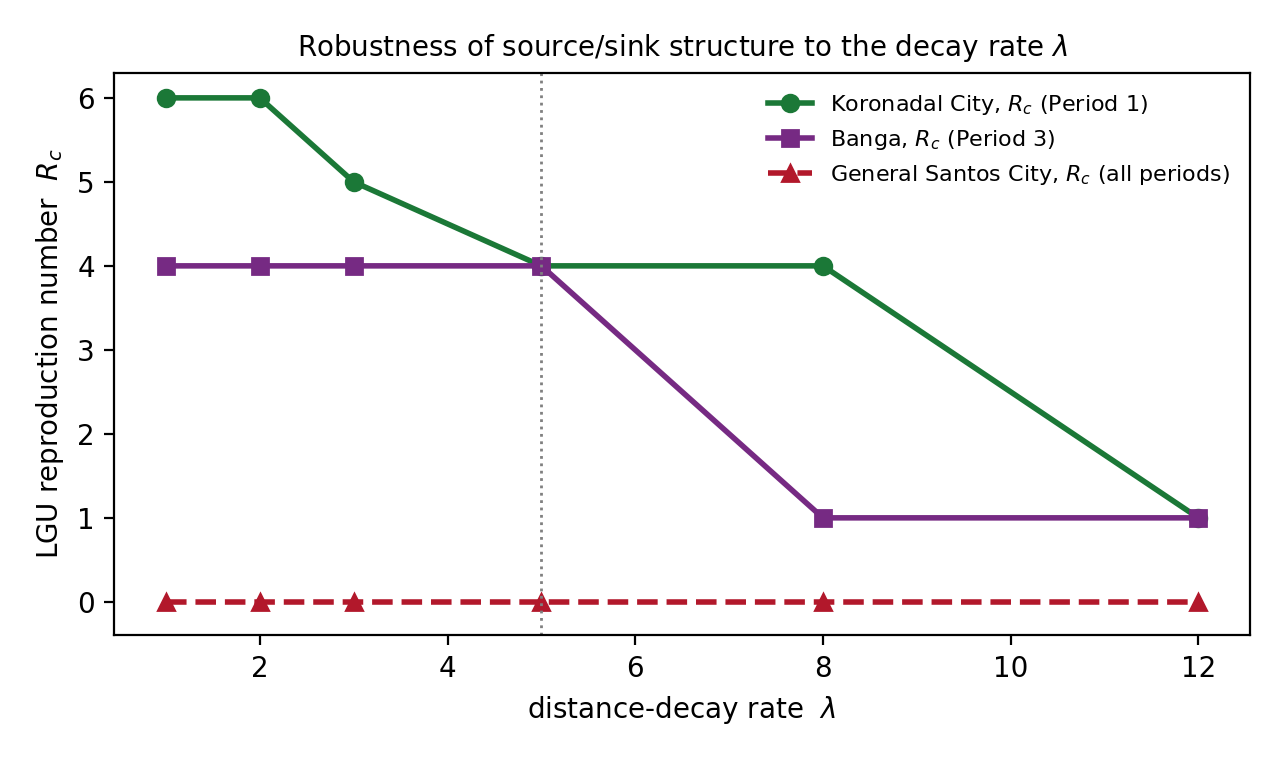
\includegraphics[width=0.62\textwidth]{kernel_robustness.png}
\caption{Leading LGU reproduction numbers as the decay rate $\lambda$ is varied
(exponential kernel, $M=5000$ realisations). Koronadal~City (Period~1) and Banga
(Period~3) persist as dominant sources while General~Santos~City remains terminal
($R_{c}=0$) at every $\lambda$; the dotted line marks the baseline $\lambda=5$.}
\label{fig:kernrob}
\end{figure}

\subsection{Preliminary cross-province transferability assessment}
\label{sec:crossprov}
To probe whether the ensemble's behaviour generalises beyond the primary study area,
we applied the identical pipeline (same $\lambda$, incubation, weights, $M$, seed,
and Strength of Linkage) to three further provinces of Region~12 drawn from the same
Department of Health line-list---North Cotabato (18 LGUs), Sultan Kudarat (12), and
Sarangani (7)---using the same three region-wide outbreak windows. In every province
the reconstruction recovers the same qualitative structure found in South Cotabato:
a single inland \emph{population/administrative hub} emerges as the dominant source,
while peripheral and coastal LGUs are terminal (Table~\ref{tab:crossprov}). The
provincial capital is the leading source in three of the four provinces
(South Cotabato: Koronadal City; North Cotabato: Kidapawan City; Sultan Kudarat:
Isulan); in Sarangani the most populous municipality (Glan) leads, with the capital
(Alabel) among the top sources. That this source/sink signature recurs across four
independent provinces, and survives changes in the LGU coordinates
(Section~\ref{sec:sens} shows the analogous robustness to the linkage weights),
indicates it is a property of the method and the settlement structure rather than of
any single dataset.

\begin{table}[htbp]
\centering
\caption{Preliminary cross-province transferability assessment: the dominant source LGU (largest
$R_{c}$, summed over the three periods) recovered by the identical pipeline in four
Region~12 provinces. \emph{These three additional provinces are a preliminary check:
municipality coordinates are GeoNames town centres (with a few estimated), the
Sultan Kudarat and Sarangani populations are provisional estimates pending official
figures, and the South Cotabato outbreak windows were reused; the numbers are
therefore indicative, not final.}}
\label{tab:crossprov}
\small
\begin{tabular}{lclc}
\toprule
\textbf{Province} & \textbf{LGUs} & \textbf{Dominant source} & \textbf{Global $R_t$ (P1/P2/P3)} \\
\midrule
South Cotabato\,$^{\dagger}$ & 12 & Koronadal City (provincial capital) & 5.0 / 2.0 / 5.0 \\
North Cotabato & 18 & Kidapawan City (provincial capital) & 2.0 / 1.2 / 2.0 \\
Sultan Kudarat & 12 & Isulan (provincial capital) & 1.4 / 1.4 / 0.5 \\
Sarangani & 7 & Glan (most populous municipality) & 1.3 / 0.8 / 0.8 \\
\bottomrule
\end{tabular}

\smallskip
\noindent\small $^{\dagger}$Primary study area (full analysis above); the other
three are the preliminary transferability assessment.
\end{table}

%======================================================================
\section{Discussion}
%======================================================================
Our aim was to identify likely sources of dengue transmission among the LGUs of
South Cotabato and General Santos City using an ensemble epidemic forest. The
clearest signal is not a fixed transmission tree but a stable partition into
sources and sinks. The provincial capital, Koronadal~City (LGU reproduction
number $R_{c}=4$ in Periods~1 and 2), and Banga in Period~3 ($R_{c}=4$) recur as
dominant sources, whereas General~Santos~City, the largest urban and coastal LGU,
is a consistent terminal recipient ($R_{c}=0$ in every period). This directional
tendency from inland population and administrative hubs toward the coastal centre
is consistent with dengue being seeded in higher-burden, earlier-onset localities and
carried onward through human mobility \cite{Stoddard2009,Wesolowski2015}, and it
is recovered here at the administrative scale at which detection and response are
organised under RA~11332 \cite{RA11332,DOH2020IRR}. At the same time, the ensemble
shows that individual parent--child links are often weakly determined, so we frame
these results as identifying priority \emph{source LGUs} for intervention rather
than as a precise reconstruction of transmission routes.

The consistently terminal position of General~Santos~City warrants comment, since
it is the largest and most connected LGU in the study area and might be expected to
\emph{export} rather than only receive infection. Three features of the
reconstruction account for the $R_{c}=0$ result, which holds in every period and
every weight combination---and, as Section~\ref{sec:sens} shows, under every decay
rate, kernel form, and the deterministic adjacency we examined (Table~\ref{tab:kernrob}). First, direction is inferred from relative onset timing,
prevalence, and proximity: across periods the smoothed epidemic in General~Santos
tends to rise \emph{after} those of the inland hubs, so the Strength of Linkage
assigns it as a recipient---most often of adjacent Polomolok---rather than a source.
Second, being terminal concerns the \emph{timing} of seeding, not the magnitude of
burden; a populous LGU can carry many cases yet still onset later than its inland
neighbours and so appear as a net importer. Third, the connectivity model uses
straight-line distance, which represents General~Santos essentially through its
nearest neighbour and cannot capture the longer-range road, commuter, and commercial
links by which a coastal hub might re-seed the interior. We therefore read the result
as indicating that, at the administrative scale and temporal resolution analysed,
General~Santos sits at the downstream end of an inland-to-coastal gradient---while
noting that this is the single finding most sensitive to the distance assumption, and
that a mobility- or transport-informed network could yet reveal a re-export role that
Euclidean coupling and LGU-level aggregation mask. We flag it as a priority for the
mobility-based extension discussed below.

Independent evidence supports this inland-hub reading. A spatio-temporal
scan-statistic analysis of dengue in the same province over 2020--2022 identified its
dominant high-incidence cluster as covering the entire municipalities of Banga, Tupi,
and Koronadal~City (relative risk $1.78$, $p<0.001$), attributing the urban centre's
elevated incidence to inadequate drainage and domestic water storage \cite{Ygona2025}.
These three municipalities are precisely those our ensemble identifies as the
province's source LGUs---Koronadal~City the dominant source in Periods~1--2, Banga in
Period~3, with Tupi a consistent secondary source---reached by a different method
(spatial cluster detection versus directional forest reconstruction) and on a
non-overlapping, earlier window (2015--2019). Because their scan statistic measures
where incidence concentrates rather than the direction of spread, the two analyses
agree on \emph{where} provincial dengue is centred even though only ours assigns a
direction to it; that convergence strengthens the case that these inland hubs---Koronadal~City
chief among them---are persistent dengue centres rather than artefacts of any single
outbreak or model choice.

Beyond South Cotabato, applying the identical pipeline to three further Region~12
provinces recovers the same qualitative structure (Section~\ref{sec:crossprov}): an
inland population or administrative hub---most often the provincial capital---emerges
as the dominant source, with peripheral and coastal LGUs terminal. That this
signature recurs across provinces of differing size and geography, and is stable
under changes in the LGU coordinates and the linkage weights, suggests it reflects
the method and the region's settlement structure rather than any single dataset. We
stress that this cross-province analysis is \emph{preliminary}: it uses
gazetteer-derived coordinates, provisional populations for two provinces, and reused
outbreak windows, and is therefore best read as a generalisability check to be
confirmed with province-specific windows and authoritative geographic and
demographic metadata.

Methodologically, the study builds directly on the region-scale epidemic forest of
Nasution et al.\ \cite{Nasution2024}, which adapted the individual-level framework
of Li et al.\ \cite{Li2019} to aggregated units and introduced prevalence as a
linkage criterion. Our departure is twofold: the fixed binary adjacency structure
is replaced by a probabilistic distance-decay connectivity network
(Eq.~\ref{eq:network}), and the forest is reconstructed as a Monte~Carlo ensemble
whose per-edge stability quantifies linkage uncertainty. Reporting stability,
rather than a single tree, guards against over-interpreting any one reconstruction
and should be standard whenever epidemic forests are built from aggregate
surveillance. The robustness analysis makes this concrete: a fixed deterministic
adjacency---the single-tree counterpart of our network---recovers the same
reproduction ratios ($R_t=5/2/5$) yet, by construction, assigns every edge a stability
of one, whereas the ensemble reveals that many of those same edges are in fact
uncertain (mean modal stability $\approx0.53$; Section~\ref{sec:sens}). Reporting a
single deterministic forest would thus present as certain what the data leave
undetermined---precisely the over-confidence the ensemble is designed to expose. Two directions follow naturally. First, because we deliberately
reconstruct at the LGU scale, our links describe coupling between administrative
units rather than between individuals; where line-list data exist, a multi-scale
reconstruction that nests individual-level trees within the LGU-level forest
\cite{LiShi2020} would let the two scales validate one another and test whether the inland-to-coastal
source--sink tendency reported here survives disaggregation. Second, the distance-decay network
could be replaced by an empirical mobility or transport network, converting the
connectivity assumption into a data-driven input.

%======================================================================
\section{Limitations}
%======================================================================
Several limitations qualify these results, some of which we encountered directly in
the course of the analysis. First, the reconstruction is \emph{unsupervised}: no
observed transmission network exists against which to validate it, so the method
identifies plausible source LGUs rather than verified routes. Individual
parent--child links are frequently weakly determined---many modal edges have
stability below $40\%$---which is why we interpret the stable source/sink partition
and reproduction numbers rather than any single reconstructed tree. Second,
aggregation to the LGU scale means the links describe coupling between administrative
units, not between individuals, and the Richards onset estimate is less reliable for
LGUs with few cases or a weak epidemic signal. Third, the identity of the dominant
source depends on modelling choices---the Strength-of-Linkage weights and the
distance-decay kernel; we probe this with the robustness analyses of
Section~\ref{sec:sens} (the source/sink partition is stable across weight
combinations, decay rates spanning an order of magnitude, a Gaussian kernel, and a
deterministic adjacency), but an empirically calibrated mobility network would still
be preferable to the assumed kernel.
Fourth, the analysis inherits the limitations of passive surveillance: under-reporting
and occasional mis-location of cases, and report-based onset dates. Fifth,
reproducing the onset estimates exactly across software was non-trivial---a Python
re-implementation of the MATLAB Sobol/optimiser routine did not bit-match, so the
primary analysis retains the original onsets while the three additional provinces use the
Python-native estimates. Finally, the cross-province transferability assessment
(Section~\ref{sec:crossprov}) is explicitly \emph{preliminary}: it relies on
gazetteer-derived town-centre coordinates rather than polygon centroids, on
provisional populations for two provinces, and on outbreak windows carried over from
the primary study area; confirming it requires authoritative geographic and
demographic metadata and province-specific period selection.

%======================================================================
\section{Conclusion}
%======================================================================
We adapted the region-scale epidemic forest to city-level dengue surveillance in
South Cotabato and General Santos City, replacing a fixed adjacency structure with
a probabilistic connectivity network and an ensemble reconstruction that
quantifies linkage uncertainty. Across three outbreak periods the method does not
recover a single fixed transmission tree, but it does recover a stable partition
into sources and sinks: the provincial capital Koronadal City (then Banga in the
third period) recurs as the dominant source, and General Santos City is a
consistent terminal recipient. This partition is robust to the linkage-weight
choice and is independently corroborated by a scan-statistic cluster analysis of
the province \cite{Ygona2025}. A preliminary application of the same pipeline to
three further Region~12 provinces recovers the same inland-hub-to-periphery
signature, indicating that the approach generalises beyond the primary study area,
pending confirmation with authoritative geographic and demographic metadata.
Because the analysis operates at the LGU scale of surveillance and response, these
source LGUs are directly actionable priority targets for dengue control, and the
reported edge stabilities make the associated uncertainty explicit.

%======================================================================
\section*{Acknowledgements}
%======================================================================
Maria Yulita Trida Tahu and Kamal Khairudin Sukandar gratefully acknowledge the
Indonesian Endowment Fund for Education (LPDP) for doctoral scholarships.

\section*{Disclosure statement}
No potential conflict of interest was reported by the author(s).

\section*{Funding}
The authors report there is no funding associated with the research featured in
this article.

\section*{Code and data availability}
The complete analysis pipeline is provided as a documented Jupyter notebook
(\texttt{epidemic\_\allowbreak forest\_\allowbreak pipeline\allowbreak.ipynb}) that reproduces every figure, table, and
reported number from the Department of Health daily case workbook and the
intermediate files it generates. The notebook implements the smoothing, onset
estimation, probabilistic connectivity network, ensemble reconstruction, and the
weight-sensitivity analysis of Section~\ref{sec:sens}, under a fixed random seed.
The code, together with the aggregated LGU-level intermediates required to reproduce
the analysis, is openly available at
\url{https://github.com/jparcede/dengue-epidemic-forest}. LGU-level dengue counts
were obtained from the Department of Health Center for Health Development XII
line-list for Region~12; the underlying case register is available from the
corresponding author on reasonable request, subject to applicable restrictions.
Population figures are from the Philippine Statistics Authority \cite{PSA2015}.

%======================================================================
\section*{Nomenclature}
%======================================================================
\begin{tabular}{ll}
$o_i$ & Onset day of LGU $i$ (days from period start) \\
$\theta_i$ & Outbreak threshold for LGU $i$ (cases) \\
$N_i$ & Population of LGU $i$ \\
$\lambda$ & Distance-decay rate in the connectivity network \\
$d_{ij}$ & Distance between LGUs $i$ and $j$ \\
$p_j(o_c)$ & Prevalence of LGU $j$ at the child's onset time \\
$\alpha,\beta$ & Weights for spatial and temporal terms in the Strength of Linkage \\
$M$ & Number of network realisations in the ensemble \\
$R_t$ & Case reproduction ratio for period $t$ \\
$R_{c,i}$ & LGU reproduction number (out-degree) of LGU $i$ \\
\end{tabular}

%======================================================================
\appendix
\section{Strength of Linkage: construction and normalisation}
\label{app:sol}
%======================================================================
This appendix derives the Strength of Linkage (Eq.~\ref{eq:sol}) used to select a
parent for each child LGU, following Nasution et al.\ \cite{Nasution2024}. Fix a
child LGU $c$ with onset $o_c$, and let $J_c$ be its admissible candidate parents
(network neighbours in the current realisation whose onset precedes $o_c$ by more
than the incubation period). Three raw quantities describe each candidate
$j\in J_c$:
\begin{itemize}
\item the \emph{spatial distance} $d_{cj}$ (Euclidean, between centroids);
\item the \emph{temporal gap} $\Delta o_{cj}=o_c-o_j>0$ (earlier candidates have a
larger gap);
\item the \emph{prevalence} $p_j$ of candidate $j$ at the child's onset time, with
$p_c$ the child's own prevalence.
\end{itemize}

\noindent\textbf{Scaling to dimensionless criteria.} Because the three quantities
have different units, each is scaled to be dimensionless. Distances are normalised
by their candidate-set \emph{minimum},
\begin{equation}
\tilde d_{cj}=\frac{d_{cj}}{\min_{k\in J_c} d_{ck}},\qquad
\widetilde{\Delta o}_{cj}=\frac{o_c-o_j}{\min_{k\in J_c}(o_c-o_k)},
\label{eq:app-norm}
\end{equation}
so that $\tilde d_{cj},\widetilde{\Delta o}_{cj}\ge 1$, with equality for the
nearest (respectively, most recent) candidate. Prevalence is scaled as a signed,
normalised difference,
\begin{equation}
\tilde p_{j}=\frac{p_j-p_c}{\max_{k\in J_c}\lvert p_k-p_c\rvert}\in[-1,1],
\label{eq:app-prev}
\end{equation}
which is largest for the candidate whose prevalence most exceeds the child's.
Equations~\eqref{eq:app-norm}--\eqref{eq:app-prev} are exactly Eqs.~(2)--(4) of
Nasution et al.\ \cite{Nasution2024}.

\noindent\textbf{Combined criterion.} The Strength of Linkage combines the three,
weighted by $\alpha,\beta$ and $1-\alpha-\beta$ (spatial, temporal, prevalence),
using the \emph{inverses} of the normalised distances so that nearer and more
recent candidates score higher:
\begin{equation}
\mathrm{SoL}_{cj}=\alpha\,\frac{1}{\tilde d_{cj}}
+\beta\,\frac{1}{\widetilde{\Delta o}_{cj}}
+(1-\alpha-\beta)\,\tilde p_{j}.
\label{eq:app-sol}
\end{equation}
Each inverse term lies in $(0,1]$ and equals $1$ for the closest/most-recent
candidate; the prevalence term rewards higher-prevalence candidates. The parent is
the candidate that \emph{maximises} $\mathrm{SoL}_{cj}$
(Eq.~\ref{eq:parent}), i.e.\ the spatially closest, temporally nearest, and
highest-prevalence admissible neighbour, traded off by the weights.
Equation~\eqref{eq:app-sol} is identical to Eq.~(5) of Nasution et al.\
\cite{Nasution2024}; adopting it lets the region-scale (Jakarta) and city-scale
(South Cotabato) studies share a single linkage definition.

\noindent\textbf{Note on an alternative parameterisation.} The accompanying code
also implements an earlier, related form in which the distances are normalised by
their candidate-set \emph{mean} rather than minimum, prevalence enters as an inverse
term, and the parent is chosen by \emph{minimisation} (selected via a configuration
flag). That variant, used during development, yields a related but not identical
source--sink partition; all results reported here use the harmonised
form~\eqref{eq:app-sol}.

%======================================================================
\begin{thebibliography}{99}
%======================================================================
\bibitem{Ong2022} Ong EP, Obeles AJT, Ong BAG, Tatengco OAG. Perspectives and lessons from the Philippines' decades-long battle with dengue. Lancet Reg Health West Pac. 2022;24:100505.
\bibitem{Undurraga2017} Undurraga EA, Edillo FE, Erasmo JNV, et al. Disease burden of dengue in the Philippines: adjusting for underreporting. Am J Trop Med Hyg. 2017;96(4):887--898.
\bibitem{Bravo2014} Bravo L, Roque VG, Brett J, Dizon R, L'Azou M. Epidemiology of dengue disease in the Philippines (2000--2011): a systematic literature review. PLoS Negl Trop Dis. 2014;8(11):e3027.
\bibitem{Edillo2015} Edillo FE, Halasa YA, Largo FM, et al. Economic cost and burden of dengue in the Philippines. Am J Trop Med Hyg. 2015;92(2):360--366.
\bibitem{Stoddard2009} Stoddard ST, Morrison AC, Vazquez-Prokopec GM, et al. The role of human movement in the transmission of vector-borne pathogens. PLoS Negl Trop Dis. 2009;3(7):e481.
\bibitem{Wesolowski2015} Wesolowski A, Qureshi T, Boni MF, et al. Impact of human mobility on the emergence of dengue epidemics in Pakistan. Proc Natl Acad Sci U S A. 2015;112(38):11887--11892.
\bibitem{Nunes2014} Nunes MRT, Palacios G, Faria NR, et al. Air travel is associated with intracontinental spread of dengue virus serotypes 1--3 in Brazil. PLoS Negl Trop Dis. 2014;8(4):e2769.
\bibitem{Stoddard2013} Stoddard ST, Forshey BM, Morrison AC, et al. House-to-house human movement drives dengue virus transmission. Proc Natl Acad Sci U S A. 2013;110(3):994--999.
\bibitem{RA11332} Philippines. Republic Act No. 11332. An Act Providing Policies and Prescribing Procedures on Surveillance and Response to Notifiable Diseases, Epidemics, and Health Events of Public Health Concern. April 26, 2019.
\bibitem{DOH2020IRR} Philippines Department of Health. The 2020 Revised Implementing Rules and Regulations of Republic Act No. 11332. 2020.
\bibitem{PSA2015} Philippine Statistics Authority. 2015 Census of Population. March 18, 2015.
\bibitem{Morales2019} Morales I, Salje H, Saha S, Gurley ES. Seasonal distribution and climatic correlates of dengue disease in Dhaka, Bangladesh. Am J Trop Med Hyg. 2019;94(6):1359--1361.
\bibitem{Polwiang2020} Polwiang S. The time series seasonal patterns of dengue fever and associated weather variables in Bangkok (2003--2017). BMC Infect Dis. 2020;20:208.
\bibitem{Maidana2007} Maidana NA, Yang HM. A spatial model to describe the dengue propagation. Trends Comput Appl Math. 2007;8(1):83.
\bibitem{Maidana2008} Maidana NA, Yang HM. Describing the geographic spread of dengue disease by traveling wave. Math Biosci. 2008;215(1):64--72.
\bibitem{Aguiar2022} Aguiar M, Anam V, Blyuss KB, et al. Mathematical models for dengue fever epidemiology: a 10-year systematic review. Phys Life Rev. 2022;40:65--92.
\bibitem{Triska2022} Triska A, Gunawan AY, Nuraini N. Outbreak spatial pattern formation based on an SI model with the infected cross-diffusion term. J Math Comput Sci. 2022;27(1):1--17.
\bibitem{Lezama2018} Lezama JAF, Vega RAM, Morales PAK, et al. Day-to-day population movement and the management of dengue epidemics. Bull Math Biol. 2018;78:2011--2033.
\bibitem{Lourenco2013} Lourenco J, Recker M. Natural, persistent oscillations in a spatial multi-strain disease system with application to dengue. PLoS Comput Biol. 2013;9(10):e1003308.
\bibitem{Nakhapakorn2006} Nakhapakorn K, Jirakajohnkool S. Temporal and spatial autocorrelation statistics of dengue fever. Dengue Bull. 2006;30:177--183.
\bibitem{Haydon2003} Haydon DT, Chase-Topping M, Shaw DJ, et al. The construction and analysis of epidemic trees with reference to the 2001 UK foot-and-mouth outbreak. Proc R Soc Lond B Biol Sci. 2003;270(1511):121--127. \url{https://doi.org/10.1098/rspb.2002.2191}
\bibitem{Li2019} Li M, Shi X, Li X, Ma W, He J, Liu T. Epidemic forest: a spatiotemporal model for communicable diseases. Ann Am Assoc Geogr. 2019;109(3):812--836. \url{https://doi.org/10.1080/24694452.2018.1511413}
\bibitem{Nasution2024} Nasution YN, Sitorus MY, Sukandar KK, Nuraini N, Apri M, Salama N. The epidemic forest reveals the spatial pattern of the spread of acute respiratory infections in Jakarta, Indonesia. Sci Rep. 2024;14:7619. \url{https://doi.org/10.1038/s41598-024-58390-3}
\bibitem{LiShi2020} Li M, Shi X, Li X. Integration of spatialization and individualization: the future of epidemic modelling for communicable diseases. Ann GIS. 2020;26(3):219--226. \url{https://doi.org/10.1080/19475683.2020.1768438}
\bibitem{Ng2019} Ng TC, Wen TH. Spatially adjusted time-varying reproductive numbers: understanding the geographical expansion of urban dengue outbreaks. Sci Rep. 2019;9:19172. \url{https://doi.org/10.1038/s41598-019-55574-0}
\bibitem{Routledge2021} Routledge I, Unwin HJT, Bhatt S. Inference of malaria reproduction numbers in three elimination settings by combining temporal data and distance metrics. Sci Rep. 2021;11:14495. \url{https://doi.org/10.1038/s41598-021-93238-0}
\bibitem{Richards1959} Richards FJ. A flexible growth function for empirical use. J Exp Bot. 1959;10(2):290--301.
\bibitem{Johnson1967} Johnson SC. Hierarchical clustering schemes. Psychometrika. 1967;32(3):241--254.
\bibitem{Ygona2025} Ygo\~{n}a J, Deligero E, Ceballos RF. Spatio-temporal analysis of dengue in the Philippines: the case of South Cotabato. Recoletos Multidiscip Res J. 2025;13(1):33--43.
\bibitem{DOH2019epi} Department of Health (Philippines). Declaration of a national dengue epidemic. Manila: Department of Health; 6 August 2019.
\bibitem{DOH12_2019} Department of Health -- Center for Health Development XII (SOCCSKSARGEN). Dengue surveillance report, Region~12, 2019.
\end{thebibliography}

\end{document}
